\section{Results}
  % Here the results of our study, within the bounds of our study only, should be discussed - times, most effective distributions, potential reasoning as to why.
  % The next section handles the relation of this to the real world.
\subsection{Control Results}

\subsection{Main Results}

\begin{figure}[H]
  \centering
  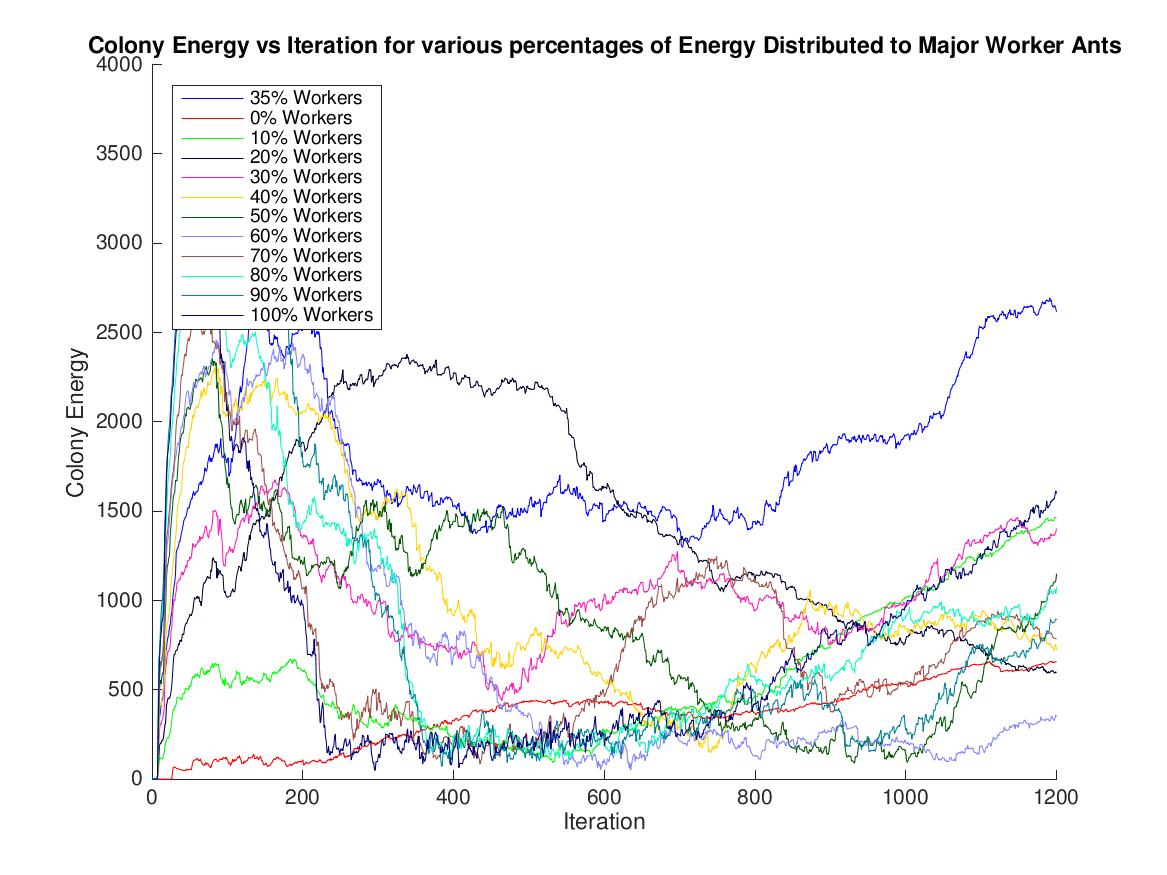
\includegraphics[width=1\textwidth]{images/line-graph-results.png}
  \caption{Line graph depicting colony energy against iterations (time) for various percentages of Major Worker Ant.}
  \label{fig:iters-line}
\end{figure}

\begin{figure}[H]
  \centering
  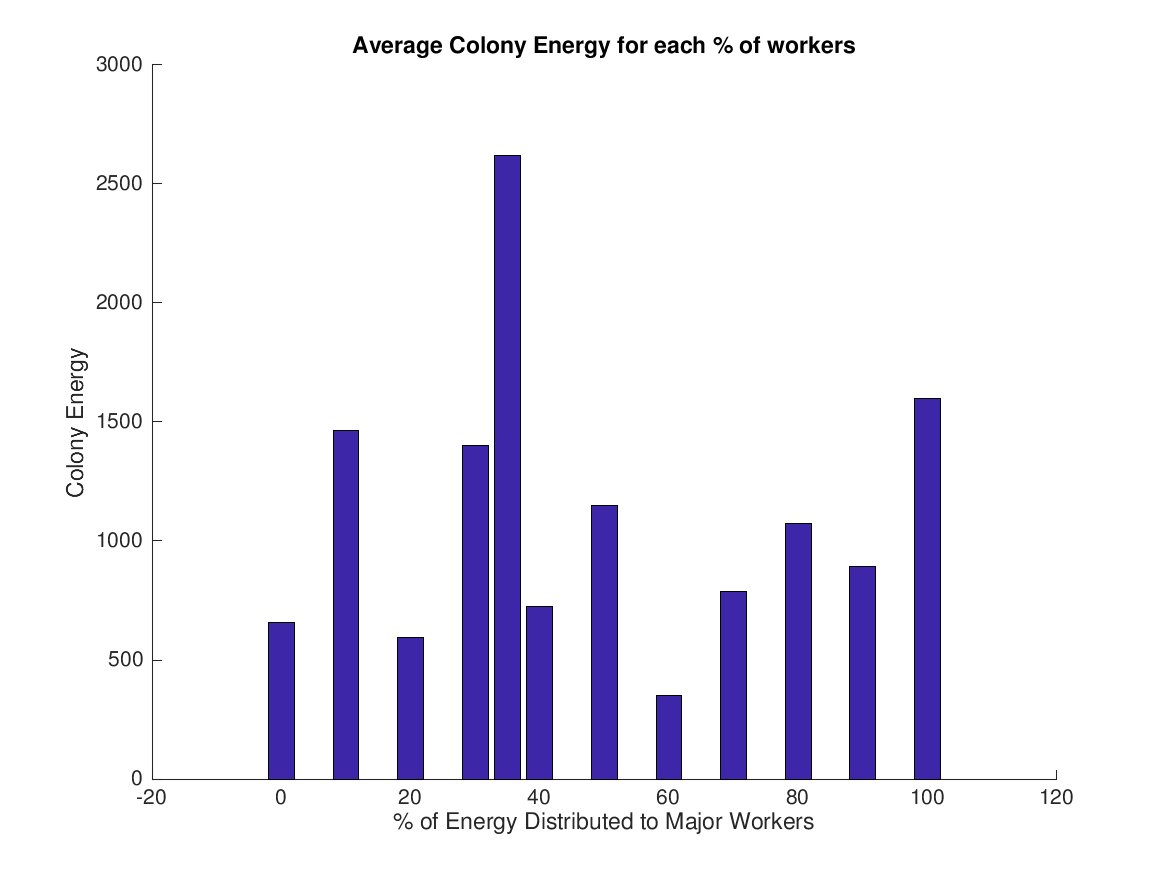
\includegraphics[width=1\textwidth]{images/bar-chart-results.png}
  \caption{Bar Chart depicting colony energy against iterations (time) for various percentages of Major Worker Ant.}
  \label{fig:iters-bar}
\end{figure}


\subsection{Computational Efficiency}

When running the simulation with graphics enabled the largest portion of computation is spent on drawing the simulations results. In order to find bottlenecks in the simulation itself the profiler was used with the graphics disabled, to give a time plot table of what functions are the most expensive during the running of an entire simulation. Appendix B, figure \ref{fig:appendix1} shows the summary of the system and figure \ref{fig:appendix2} of the same appendix shows that the environment is the place where most computation happens.\par

 \begin{figure}[htb]
  \centering
  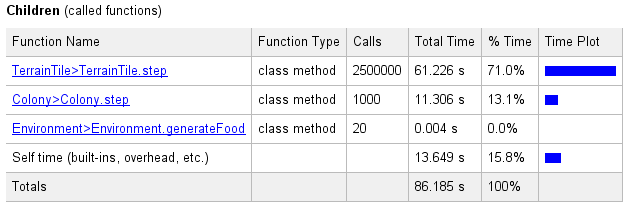
\includegraphics[width=0.8\textwidth]{images/text1.png}
  \caption{Profiling for the child functions of Environment - Environment.step}
  \label{fig:text1}
\end{figure}

 \begin{figure}[htb]
  \centering
  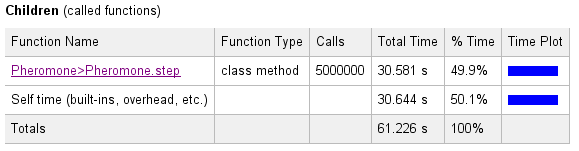
\includegraphics[width=0.8\textwidth]{images/text2.png}
  \caption{Profiling for the child functions of TerrainTile - TerrainTile.step}
  \label{fig:text2}
\end{figure}

When overviewing the computational costs of the environment step, it's highlighted in figure \ref{fig:text1} that the terrain tile is where the large majority of time is spent. As shown in figure \ref{fig:text2}, a large amount of the computation that is done during the simulation of the terrain tile is a result of the pheromone step function. As a result, it can be seen that the pheromone step is taking a large amount of computation to run, the reason for this being so expensive is that each tile of the map contains a pheromone which is then updated each timestep of the simulation. Running it this way means that tiles without active pheromones will still be receiving updates each timestep. However, a way of improving this to greatly reduce computation would be to instead keep a list of active pheromones and then only update those inside that list. When a pheromone decays to zero strength, the pheromone can be removed from the list and won't be unnecessarily updated each timestep.\par

\subsection{Repeatability}
